Inspired by the FloPoCo\cite{8877424} project, our design methodology can best be described as \emph{computing just right}.
We aim for just the right amount of compute and abstraction for the task at hand, no more no less.
This methodology stands in contrast to the design methodologies of architecture designers for commodity hardware accelerators (such as GPUs), which aim to support a large set of use cases.
Accordingly, our methodology consists of five techniques distilled from such general purpose architectures and tools but simplified for our specific purposes.

\subsection{Abstract Interpretation for Efficient Transformations}\label{subsec:loop-unrolling}

It is well known that the way to achieve peak performance/lowest latency inference of a DNN is to linearize the control flow graph\cite{osti_1574050} (i.e., remove branches) and flatten the dataflow graph as much as possible\cite{10.1145/3295500.3356173} in order to execute as many operations in parallel as possible.
For intermediate level representations of a DNN (e.g., loops) this corresponds to loop unrolling followed by fusion (alternatively known as unroll and jam\cite{thomas1971catalogue}).
For example, consider the pair of loop nests in Listing~\ref{lst:loop_fusion}.
Note that a loop fusion pass performed by either MLIR or LLVM would verify that memory independence constraints are satisfied for all pairs of stores and loads in each of the loop nests.
Thus, after unrolling the inner loops of the second loop nest (on \mintinline{mlir}{%arg5}, \mintinline{mlir}{%arg6}, \mintinline{mlir}{%arg7}) we incur
\[
	\mathtt{\%c1} \times \mathtt{\%c3} \times \mathtt{\%c3} \times 2 \times 4
\]
memory independence checks.
This indicates that unroll and fuse optimizations take increasingly longer as one experiments with larger and larger unroll thresholds, where the \emph{unroll threshold} determines which loops will be fully unrolled (all loops with trip count less than or equal to the threshold will be unrolled).
\begin{longlisting}
	\inputminted[highlightlines={5,6,17,18,19,22}]{mlir}{sources/loop_fusion.mlir}
	\caption{Loop fusion and unrolling example, with emphasis on loads and stores whose independence must verified.}
	\label{lst:loop_fusion}
\end{longlisting}

\begin{longlisting}
	\inputminted[highlightlines={5,6,11-13,16},linenos=true,numbersep=\mintednumbersep]{mlir}{sources/unrolled_loop.mlir}
	\caption{Unrolled and fused loop, for which store-load forward can be performed.}
	\label{lst:storeloadforwarding}
\end{longlisting}

%followed by store-load forwarding or, alternatively, wholly promoting stores-loads to registers.
Following unroll and jam, we are able to perform \emph{store-load forwarding}, i.e., we are able to omit those store operations that store to memory addresses which are subsequently loaded from.
For example, consider the above loop nests fused, with the second loop nest having the inner three loops fully unrolled (see Listing~\ref{lst:storeloadforwarding}); the store operations on lines 6 and 13 can be entirely eliminated and the load operation on line 5 can be forwarded to the \mintinline{mlir}{arith.addf} on line 15.
For store-load forwarding, for each load operation that follows a store operation, the compiler must check whether the store and the load access the same location in memory, and further verify that there are no intervening store operations to the same memory address;
for store operations in the body of a loop, this requires solving the constraint system discussed in Section~\ref{subsec:mlir}.
We can clearly observe that as loops are further and further unrolled, the cost of this particular optimization grows quadratically.
This is because in a fully unrolled loop nest, with many parallel dataflows, a store operation in one dataflow might be forwarded across a parallel dataflow (and thus incur checks against all stores and loads in that parallel dataflow).

In principle, we could rely on MLIR or LLVM to perform each of these optimizations.
The chief impediment to relying on these general purpose compilers for our needs is the complexity and sophistication of the algorithms used to perform each phase of the translation in an automated way.
For general purpose programs this is an acceptable cost, especially given that most development is done without aggressive optimization in order to get fast build times in order to iterate on the logic of the program (leaving the aggressive optimization compilations for release ready builds).
For us, given that the logic and dataflow of BraggNN is fixed (having already been iterated on), and given that we are in fact searching the design space for optimal low-level representations of the DNN, the runtimes of these algorithms are prohibitive (taking on the order of hours and sometimes days to complete).
Moreover, often their rigor and conservatism are unnecessary given a high-level understanding of the structure of BraggNN; for example, in the case of fully unrolling the above loop nests and forwarding from the stores during initialization to the loads during accumulation, the region within which the forward is safe is clear from the semantics of convolutions.
The loop indices and corresponding memory addresses for these safe store-load forwards are very easy to compute analytically and ahead of time (even in the presence of complications such as strided tensors).

In order to avoid these enormously costly and unnecessarily complex optimization passes, we completely omit them.
Instead, we do not lower BraggNN past the scf dialect, and instead implement an \commnt{check this name with karthik}{abstract interpreter, which }performs the unrolling blindly (i.e., without verifying constraints) but correctly, i.e., in such a way that the unrolled loops do not perform invalid stores/loads.
In addition to efficiently unrolling loop nests, our abstract interpreter performs store-load forwarding.
We also make use of a fundamental platform differences between fixed architectures (such as CPUs or GPUs) and FPGAs, and a convenient feature of BraggNN;
namely we eliminate all stores and loads of intermediate activations (which would translate to stores and loads from Block RAM on the FPGA) to registers or wires.
Furthermore, since BraggNN is a relatively small DNN, we inline absolutely all of the weight tensors as constants and perform \emph{constant propagation}.
Finally, our abstract interpreter identifies sequences of multiplications and additions and fuses them into single operation fused-multiply-adds, i.e., our abstract interpreter emits \mintinline{mlir}{llvm.fmuladd} instructions.
By performing each of these transformations
\begin{enumerate}
	\item We completely eliminate any latency due to loading from or storing to memory for intermediate activations;
	\item We completely eliminate all logic (i.e., integer arithmetic) related to calculating memory offsets, a non-trivial reduction in instruction count and design complexity (see figure <figure> for reduction in instruction count);
	\item We are able to instantiate a reduced set of floating point operation cores (i.e., only \mintinline{mlir}{fmuladd} cores), and thus reduce complexity and overall latency of our design.
\end{enumerate}
Note, we are able to make the memory to registers transformations because BraggNN is a relatively compact DNN and our target FPGA is plentiful in registers.
The reinterpreted semantics implemented by our abstract interpreter are presented in Eqns~\eqref{eqn:semantics}.

\begin{equation}\label{eqn:semantics}
\begin{split}
	f_{Z} \llbracket x \coloneqq y + z\rrbracket (\sigma) &= [ x \mapsto Z ] (\sigma) \\
	f_{Z} \llbracket x \coloneqq y + z\rrbracket (\sigma) &= [ x \mapsto Z ] (\sigma) \\
	f_{Z} \llbracket x \coloneqq y + z\rrbracket (\sigma) &= [ x \mapsto Z ] (\sigma) \\
\end{split}
\end{equation}
%\begin{figure}
%	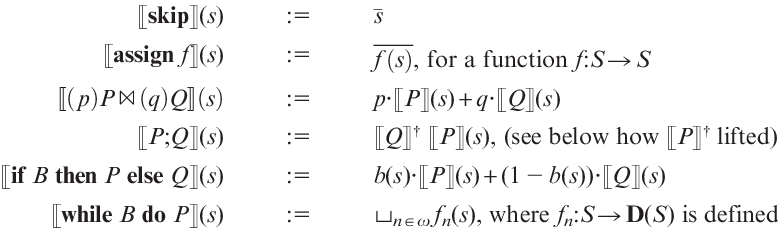
\includegraphics[width=\columnwidth]{figures/semantics}
%	\caption{This is a placeholder.}\label{fig:semantics}
%\end{figure}

\subsection{Parallel Topological Sort Scheduling}\label{subsec:parallel-toposort-scheduling}

In addition to reducing the runtime of the MLIR frontend, our abstract interpreter simplifies the LLVM IR that we pass to Vitis, and thus, in theory reduces its workload as well.
In actuality, performs these optimizations/passes ahead of time (i.e., using MLIR, LLVM, or our abstraction interpreter to unroll loops), Vitis will rerun the same or similar passes without any intervention by the user, on behalf of the user, as part of its default optimization/transformation pipeline.
Thus, a fundamental challenge in implementing BraggNN as a digital design is reducing the time taken by Vitis in performing its own optimizations.
In addition to those ultimately redundant passes, Vitis takes an inordinate amount of time to schedule the large number of operations that comprise BraggNN when fully unrolled, even after eliding unnecessary operations such as integer arithmetic associated with computing memory offset.

Thus it becomes necessary to completely eliminate Vitis and (therefore HLS) from the design flow.
Recall that the crucial task which Vitis HLS fulfills is the scheduling of operations during each clock cycle, in such a way that they respect the dataflow graph; that schedule then informs the construction of a corresponding FSM.
In general, for complex programs, this is indeed a computationally intensive task, necessitating formulating the scheduling problem (see Section~\ref{subsec:hlsdown}) and solving it using either an MIP solver or, if the problem is formulated as an SDC, an LP solver.
In the case of BraggNN, and in fact many DNNs, where the dataflow is very regular and where parallel execution is only bounded by the number of DSPs (since we eliminate the need for BRAMs by using only registers), it is straightforward to construct the optimal schedule based solely on a topological sort of the operations.

In fact, by computing the schedule "by hand", we can exercise finer control over DSP usage and thus further reduce the overall complexity of the design.
That it to say, we can schedule using the maximum number of DSPs possible during each state of the FSM, in contrast to Vitis, which attempts to make conservative use of DSPs, which leads to excessive LUT usage for muxing (as discussed in Section~\ref{subsec:hlsdown}); see figure <...> for a comparison the LUT usage using our scheduling algorithm versus Vitis' scheduling algorithm.
One thing to note here is that computing a schedule using sequential topological sort becomes costly (in terms of runtime) for the larger scalings of BraggNN, where we need to schedule upwards of 1E6 operations.
To ameliorate these costs we implement a parallelized topological sort\cite{sanders2019sequential}.
Thus, we build our schedule, bounded only by the number of available DSPs, extract the control FSM, and generate the corresponding RTL.
See Algorithm~\ref{alg:toposort} for a precise specification of our scheduling algorithm.

\begin{algorithm}
	\caption{Placeholder}\label{alg:toposort}
	\begin{algorithmic}
		\Require $n \geq 0$
		\Ensure $y = x^n$
		\State $y \gets 1$
		\State $X \gets x$
		\State $N \gets n$
		\While{$N \neq 0$}
		\If{$N$ is even}
		\State $X \gets X \times X$
		\State $N \gets \frac{N}{2}$  \Comment{This is a comment}
		\ElsIf{$N$ is odd}
		\State $y \gets y \times X$
		\State $N \gets N - 1$
		\EndIf
		\EndWhile
	\end{algorithmic}
\end{algorithm}

\subsection{Bit Twiddling Hacks}\label{subsec:bit-twiddling-hacks}

Given that we are generating RTL free of the constraints of Vitis, in addition to being able to exercise precise control over total DSP usage, we are able to exercise more precise control over how the DSPs are configured;
Vitis, due to a current bug\footnote{\url{https://support.xilinx.com/s/question/0D52E00006hpMZQSA2/vitis-hls-cannot-invoke-dspfp32-maddmacc-mode-for-versal?language=en_US}}, cannot infer fused-multiply-adds ($a \times b + c$), whereas we can directly instantiate such operations.
Using our abstract interpreters representations for sequences of multiply and add operations (see Section~\ref{subsec:loop-unrolling}), we can instantiate fused floating multiply add cores.
Thus, we instantiate the maximum number of fused-multiply-adds and map all arithmetic operations to these units.
Note that since FPGAs cannot be reconfigured at runtime\cite{reconfigfpga}, in order for this to be feasible, we must normalize all arithmetic operations in BraggNN to be in terms of a fused-multiply-add, i.e., $a \times b + c$.
For multiplications (by setting $c = 0$) and additions (by setting $b = 1$) this is straightforward.
For subtractions, we can preprocess the subtrahend by flipping the sign bit (and then set $b = 1$).
Division is the only primitive operation that presents a serious challenge to normalization in this way.
To normalize division we exploit the fact that aliasing floating point to an integer implements an approximate binary logarithm\cite{enwiki:1081681080};
we use this property to approximate the inverse (of a floating point number) and then perform division through multiplication by that inverse.
In our experiments (and prior work\cite{10.1007/978-0-387-72258-0_14}) this approximation incurs approximately a $4\%$ difference in accuracy per division.

Finally, we experiment with alternative bitwidth implementations of IEEE754 single precision floating point.
With respect to the BraggNN training, we observe that the sample data does not use a full 8 bit exponent (see Figure~\ref{fig:numexp}).
\begin{figure}
	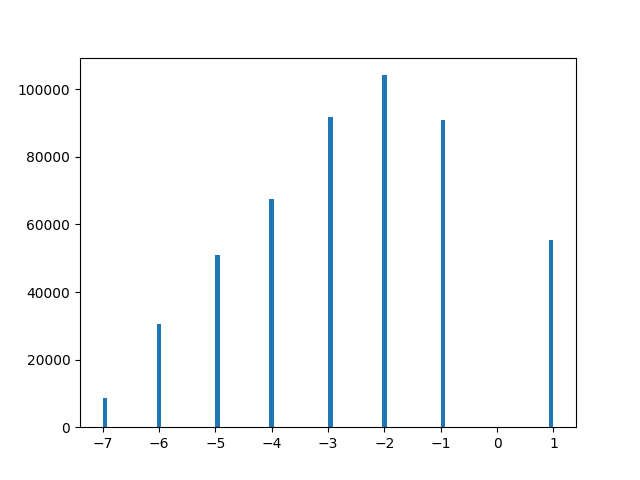
\includegraphics[width=\columnwidth]{figures/exp_bits}
	\caption{Range of exponent values for BraggNN training data.}\label{fig:numexp}
\end{figure}
To this end, we employ the FloPoCo\cite{8877424} generator of arithmetic cores to generate IEEE754 floating point fused-multiply-adds with only 3 bits for the exponent (and 23 bits for the mantissa).
This produces floating point arithmetic cores that use fewer registers and having smaller wire delays, again leading to a reduction in overall complexity and end to end latency.
